\documentclass{jhwhw}
\usepackage{amssymb,amsmath,graphicx}

\begin{document}

\title{High Performance Networks - Final Exam}
\author{Cody Boppert}

\maketitle

\section*{Final Exam}
\nopagebreak[4]

\problem{}
(20 pts) A bandwidth-limited network-layer path carrying user data is abstracted as a black-box for end-to-end rate adaption purposes. The adaptation process involves the send adjusting the data rate $\lambda$ based on  the observed loss ration $L$ (i.e. the fraction of data packets reported as lost by the receiver). An AIMD-based adaptation algorithm treats the network path as a computational function of the form: $L = \mbox{net}{\lambda}$ where $\lambda > 0$ and $L > 0$. The algorithm is cognizant of how the net($\cdots$) behaves when $\lambda$ changes, as given by the relationship:
\begin{equation*}
\mbox{net}(\lambda + \Delta) > \mbox{net}{\lambda} > \mbox{net}(\lambda - \Delta)
\end{equation*}
for $\Delta > 0$. The control steps in AIMD algorithm in invoke the net($\lambda$) function in the following way:
\subparagraph{}
Suppose $\lambda_{0}$ is an initial input for which net$(\lambda_{0})$ returns a value $L_{0} > \delta_{h}$, where $\delta_{h} > 0$. In that case, the algorithm reduces $\lambda$ in multiple steps of $(\beta \times L)$ decrements to a value $\lambda_{f}$ such that net$(\lambda_{f}) < \delta_{l}$, where $\beta > 0$ and $0 < \delta_{l} < \delta_{l}$. Thereupon, the algorithm increases $\lambda$ in  multiple steps of $\alpha$ increments to a value $\lambda_{t}$ such that net$(\lambda_{t}) > \delta_{h}$, where $\alpha > 0$. Thereafter, the decrease procedure kicks in again. Thus there is a repetitive cycle of decrease and increases of $\lambda$.\\

\noindent The control steps in the AIMD algorithm interacting with net($\cdot$) are shown in Figure 1-(a) using a C-like syntax. Figure 1-(b) shows the empirical behavior of AIMD algorithm with respect to $i$ for\footnote{The control step number $i$ as incremented in the "while" loop denotes the passage of time in the physical world, i.e., end-to-end network path, represented by the net$(\lambda)$ function.} the base values $\beta = \beta'$ and $\alpha = \alpha'$. Show an empirical graph of how $(L, \lambda)$ varies with respect to $i$ for each of the cases.

{\centering
	\includegraphics[width=500px]{./figure1.png}\par
}

\newpage
\solution
\part
$\beta > \beta', \alpha = \alpha'$ 

{\centering
	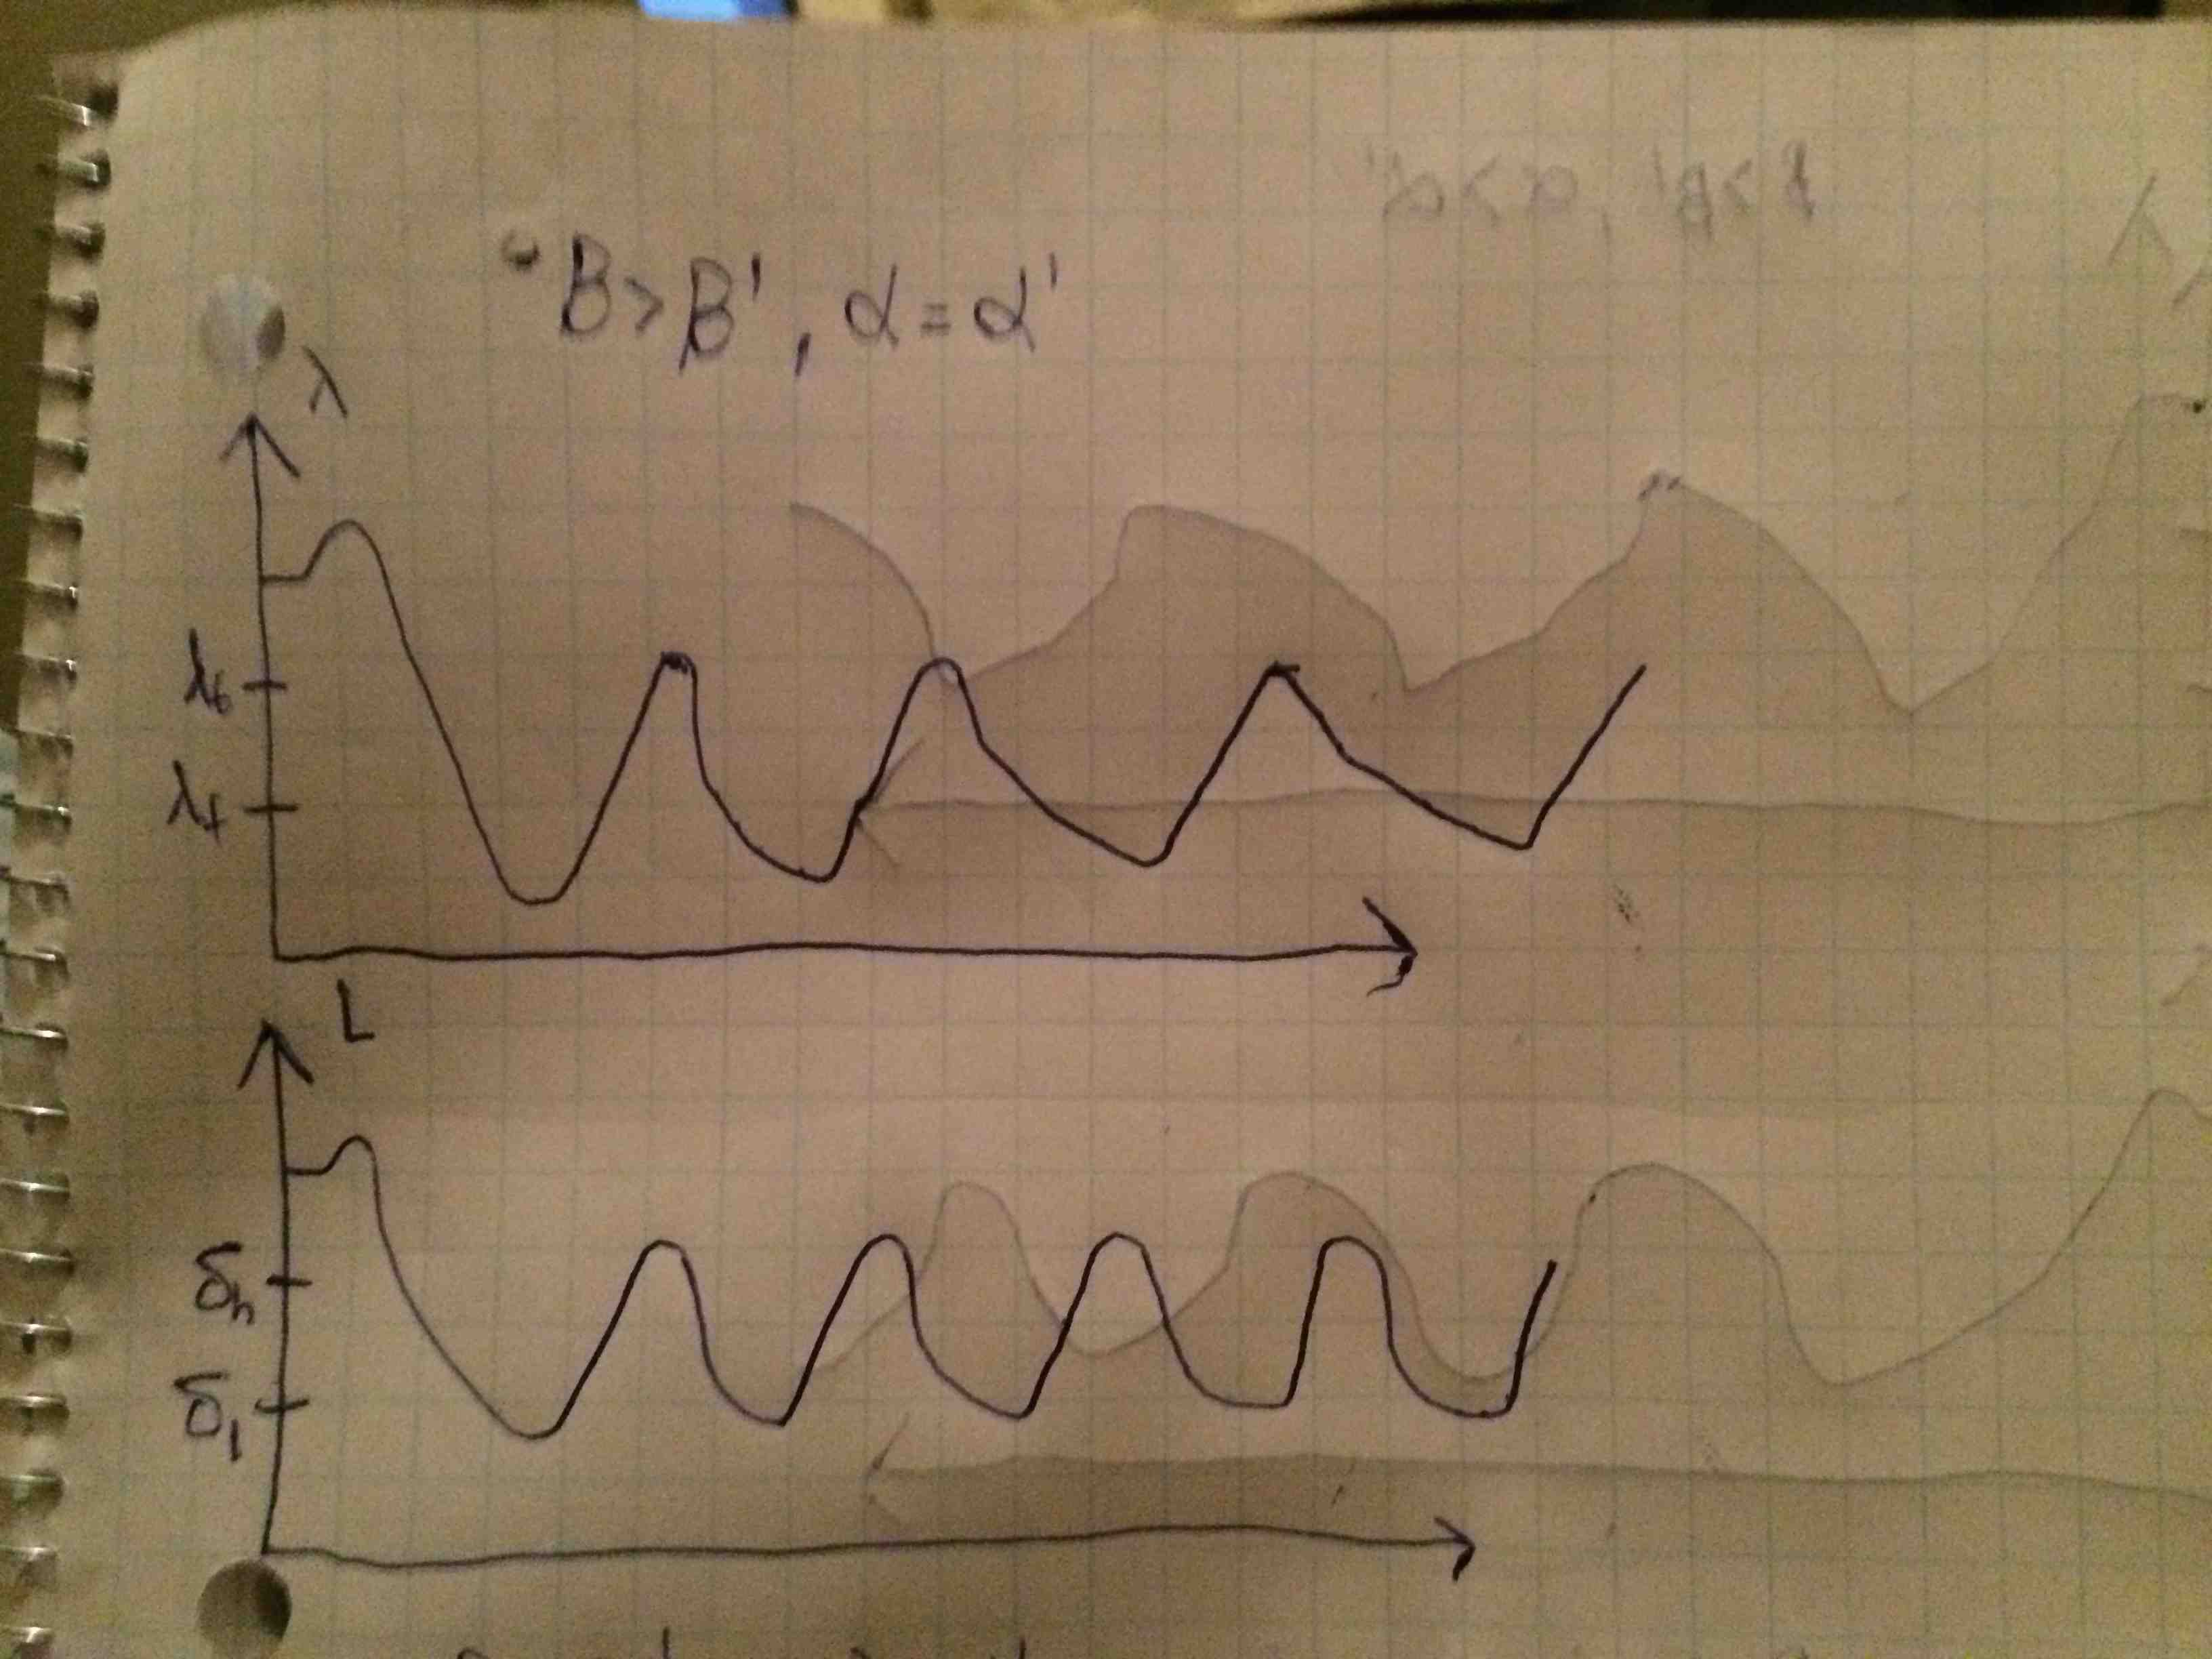
\includegraphics[width=500px]{./image3.jpg}\par
}
\noindent In this we see the decrease phase starts sharp and tails off until the linear increase phase.

\newpage
\part
$\beta = \beta', \alpha > \alpha'$

{\centering
	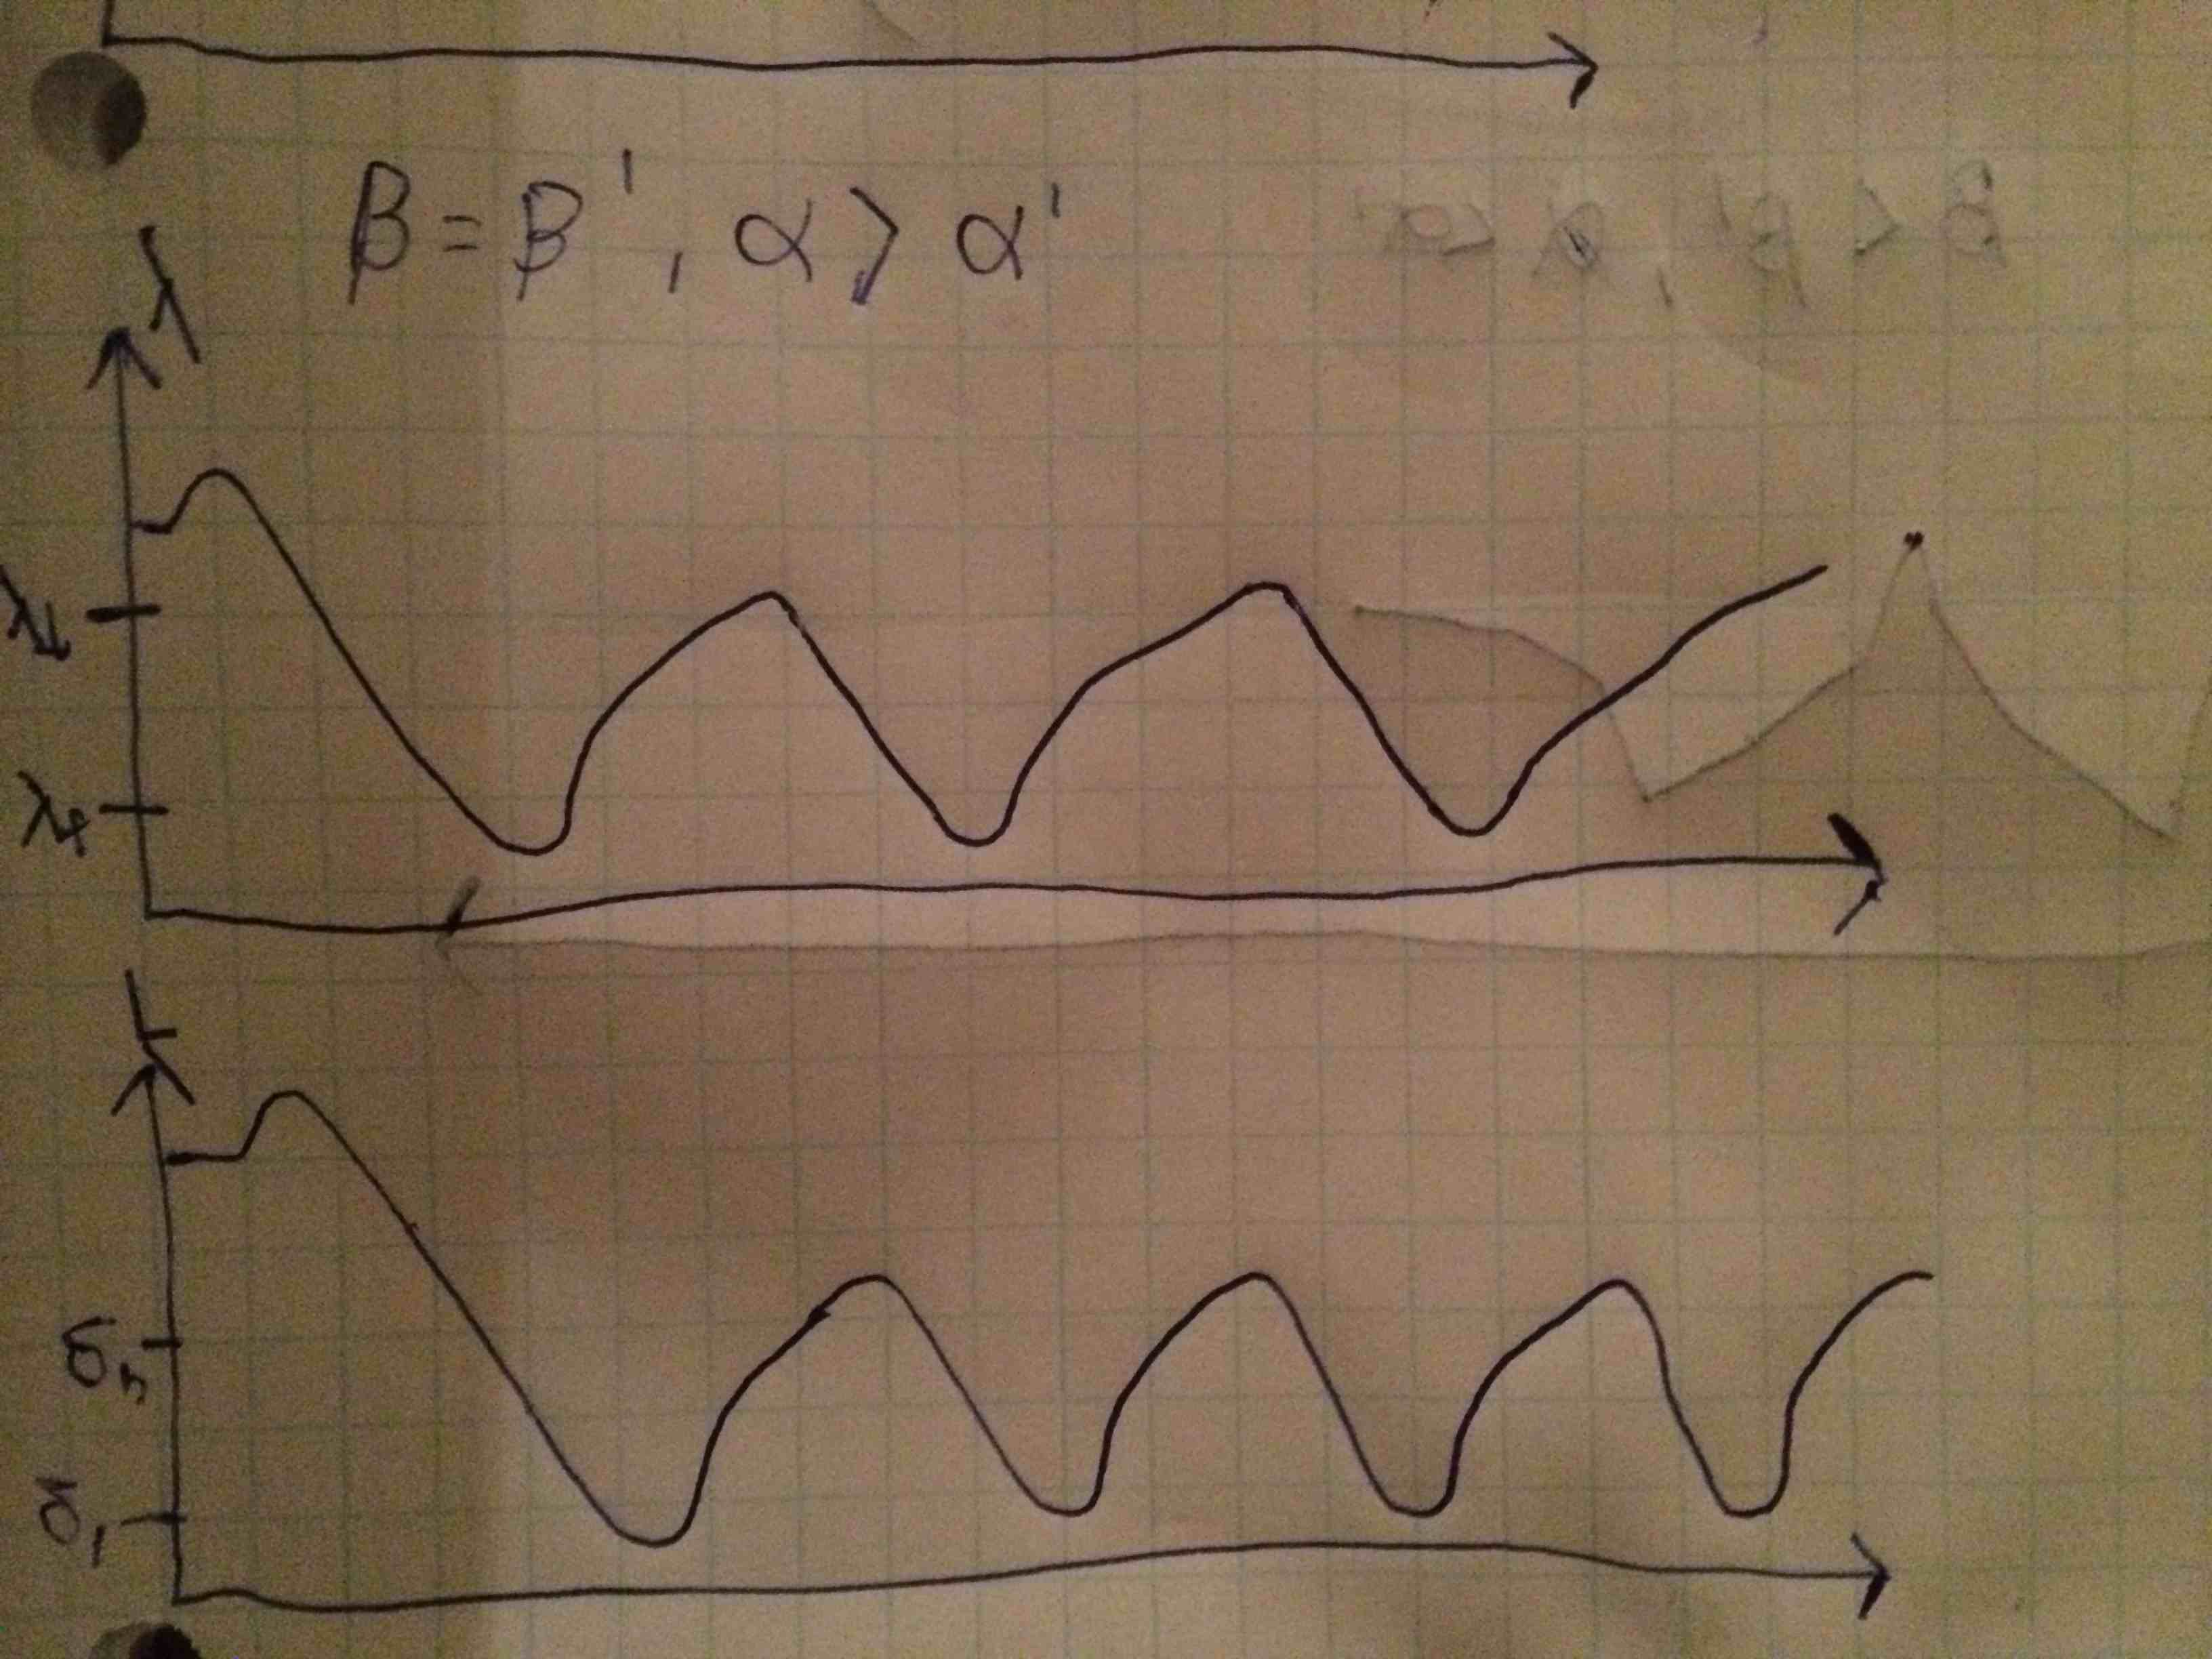
\includegraphics[width=500px]{./image4.jpg}\par
}
\noindent Here the decrease phase is linear downwards but the increase phase starts with a sharp increase and tails off as time goes on.


\newpage
\part
$\beta > \beta', \alpha > \alpha'$

{\centering
	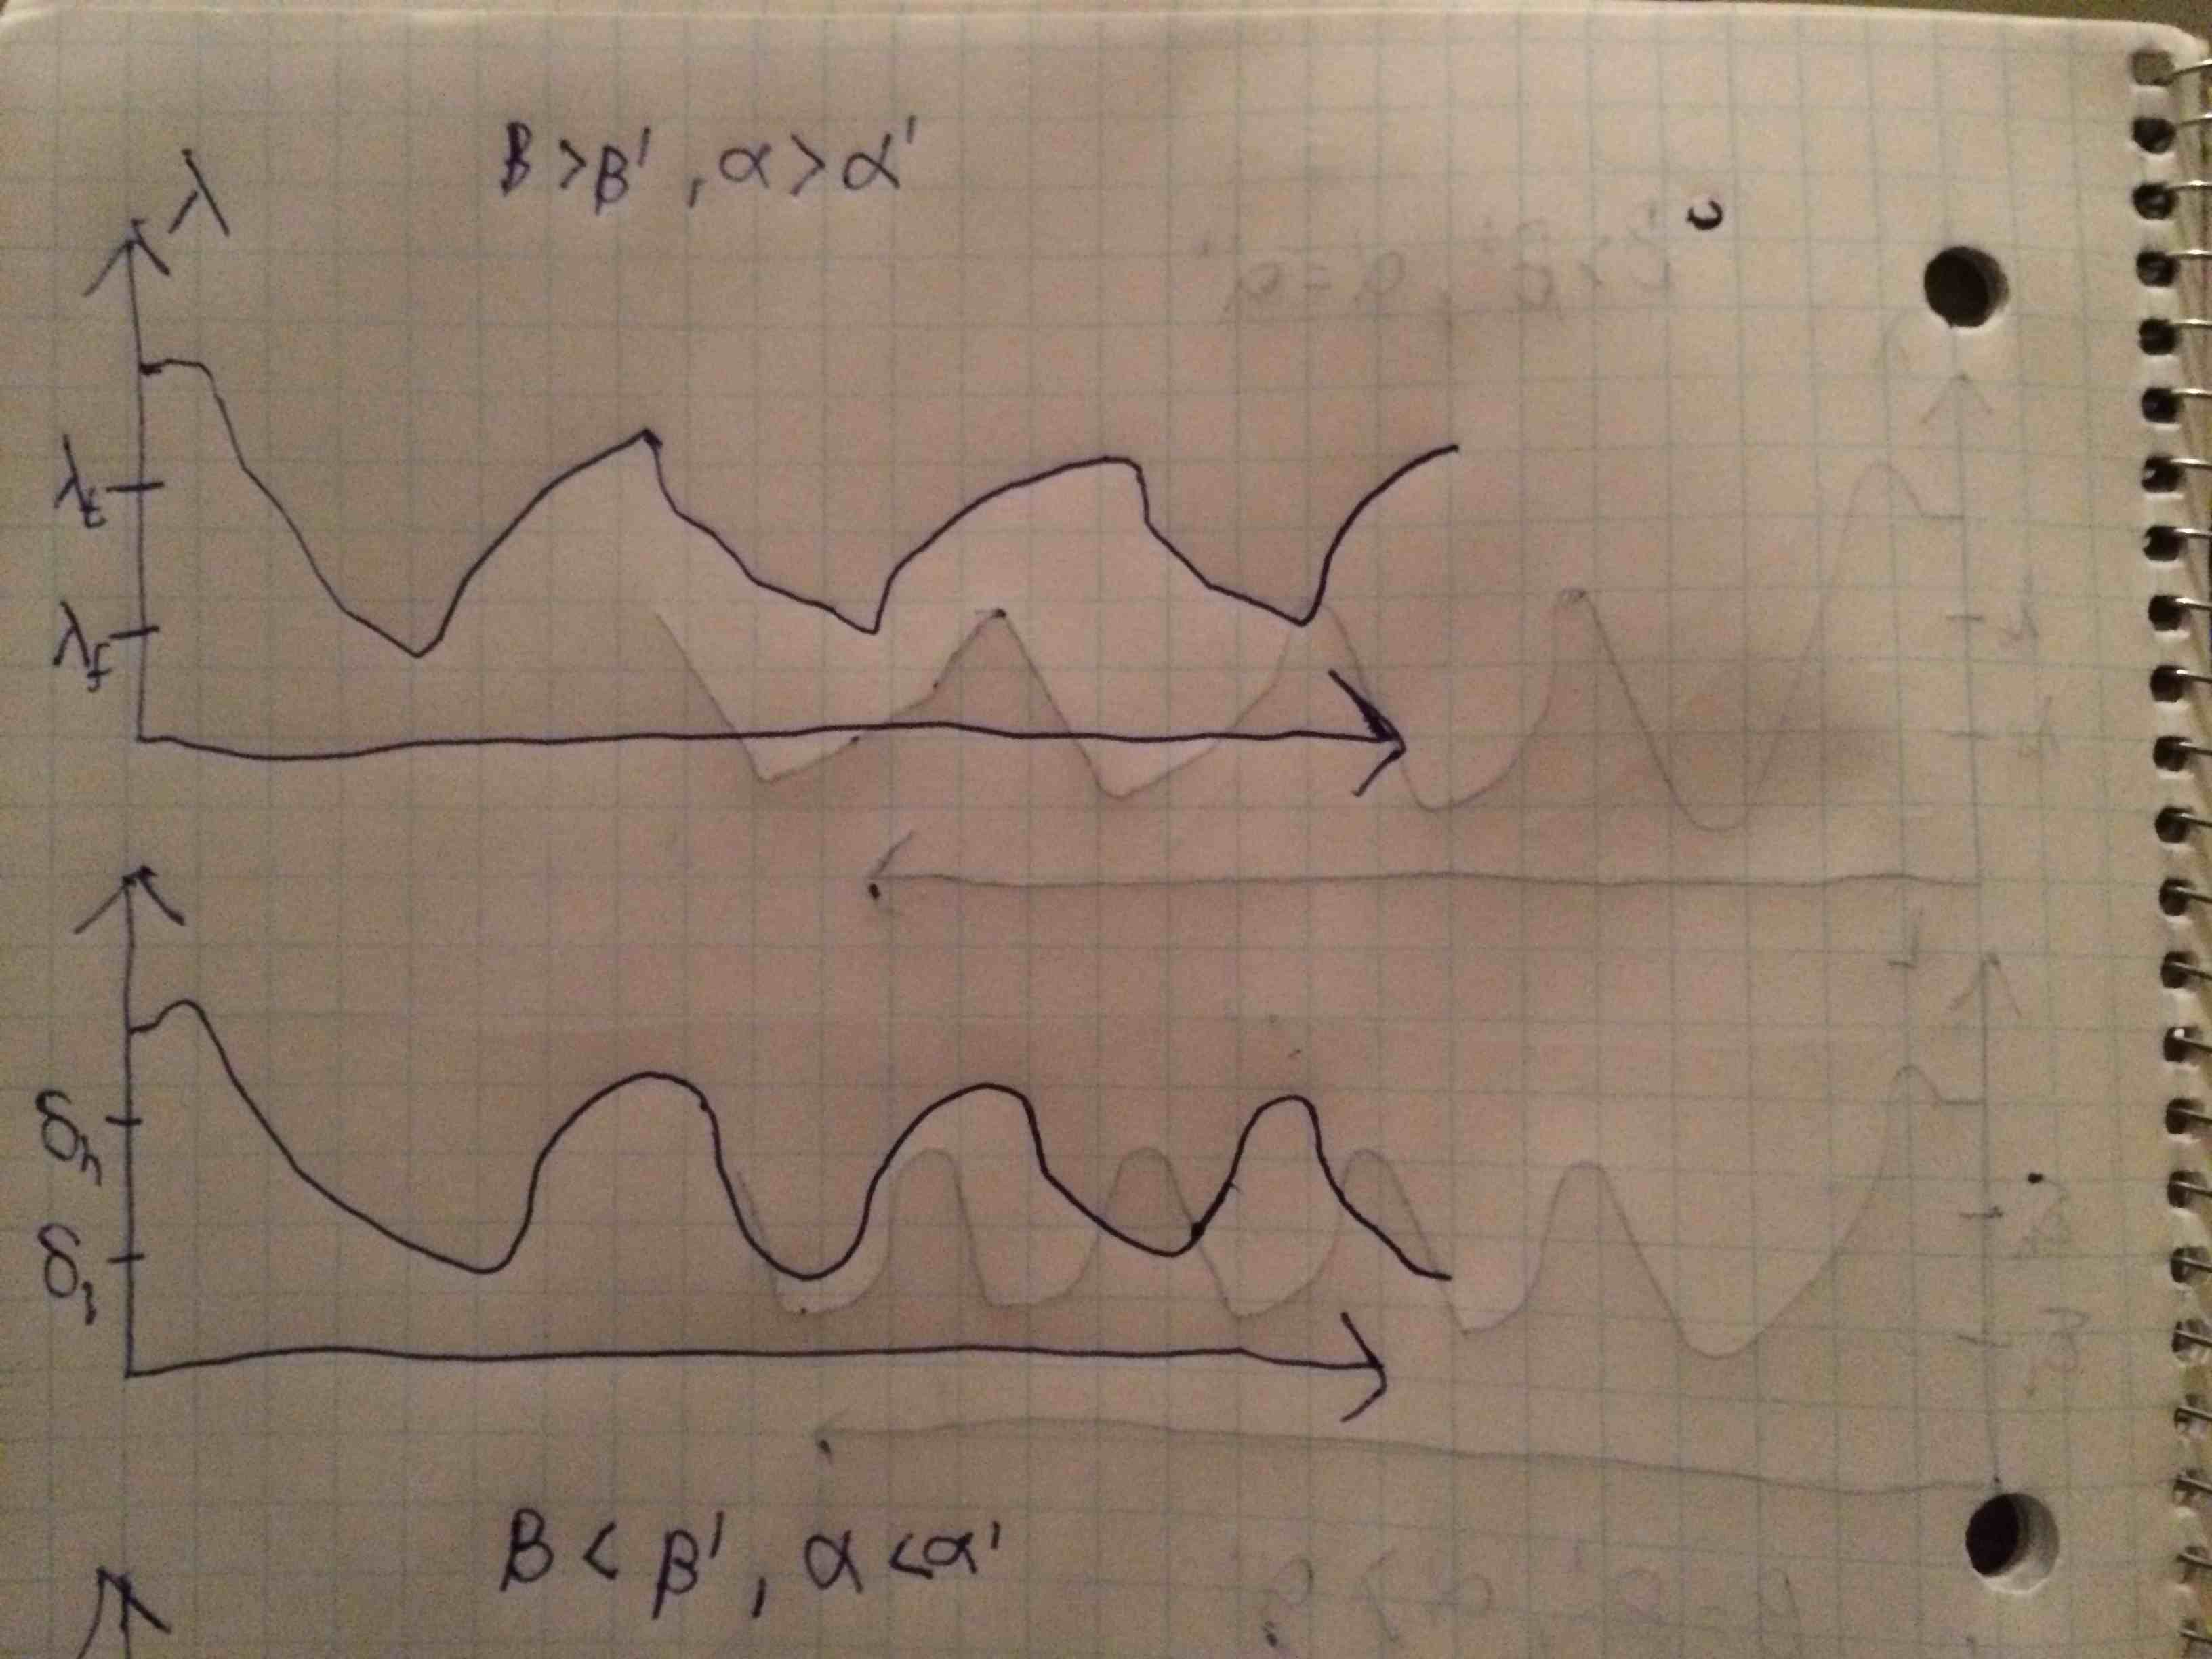
\includegraphics[width=500px]{./image.jpg}\par
}
\noindent Here both the decrease and increase phases are sharp at first and tail off towards the end.

\newpage
\part
$\beta < \beta', \alpha < \alpha'$

{\centering
	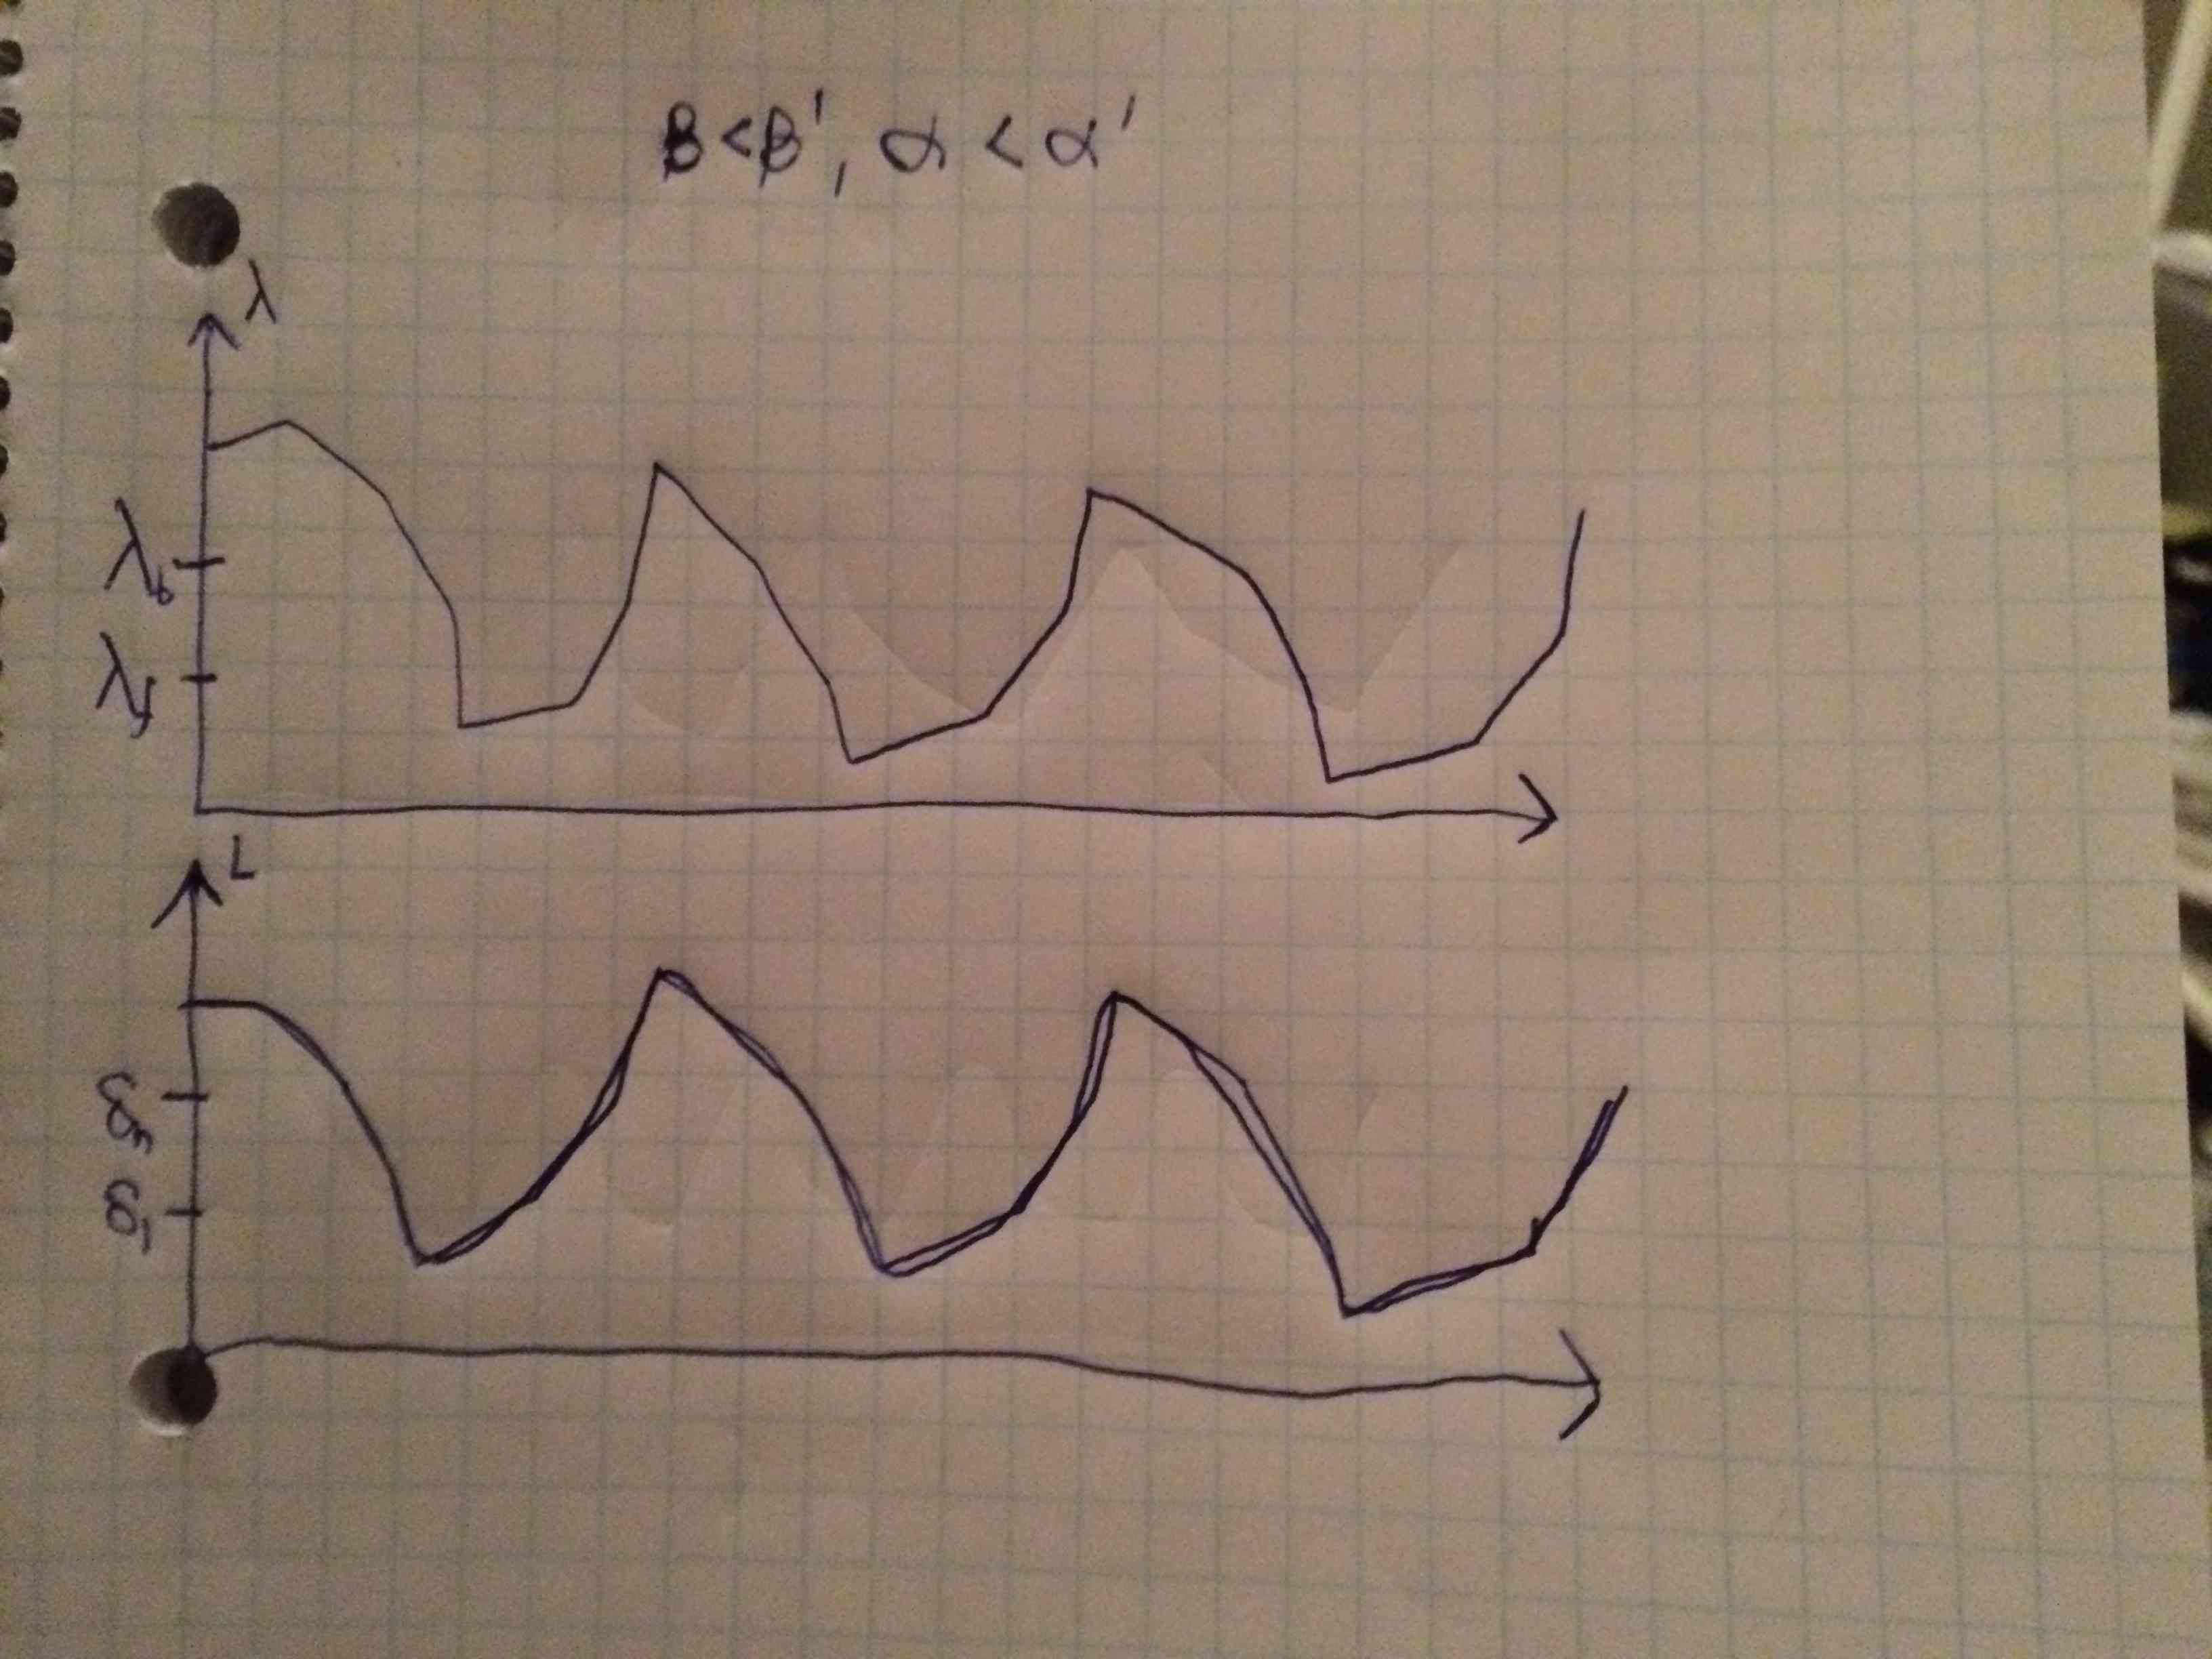
\includegraphics[width=500px]{./image2.jpg}\par
}
\noindent Here both the decrease and increase phases start off a little slower and increase in slope with tim.e

\problem{}
(15 pts) Consider the multicast delivery of packets from a source $s$ to a set of $\mathcal{N}$	receivers over a network of routers, where $\mathcal{N} \ge 1$. A multicast protocol $P_{m}$ may create a tree-structured path for carrying packets, whereby an on-tree router replicates a packet $q$ received along its incoming link to forward $q$ over its outgoing links that lead to receivers. $P_{m}$ is more efficient than a protocol $P_{u}$ that requires $s$ to send a copy of $q$ to each of the receivers separately over distinct point-to-point paths. Here, efficiency improvement of $P_{m}$ over $P_{u}$ is measured by how many less number of distinct copies of packet $q$ are transmitted along various hops in the network to effect the delivery of $q$ at all receivers (for a given source-receiver placement in the topology). Referring to Figure 2, $P_{m}$ requires $q$ to traverse 3 distinct hops, whereas $P_{u}$ requires 4 hop traversals by $q$. In general, we may express the efficiency improvement of $P_{m}$ over $P_{u}$ as:
\begin{equation*}
I = [1 - \frac{\mbox{overhead}(P_{m})}{\mbox{overhead}{P_{u}}}] = \mathbf{O}(N^{\alpha}L),
\end{equation*}
where $L$ is the diameter of the network (i.e., the maximum number of hops between any pair of nodes) and the parameter $\alpha$ factors in the topological characteristics of the distribution tree --- such as the number of network nodes and links. Explain, with reasoning, as to which of the following statements about $I$ are true.

{\centering
	\includegraphics[width=500px]{./figure2.png}\par
}

\newpage
\solution
\part
$\alpha > 1.0$ \\ 
\noindent \textbf{False}
\part
$\alpha \ge 1.0$ \\
\noindent \textbf{False}
\part
$0.0 < \alpha < 1.0$
\\ \\
\noindent \textbf{True}. This is the only true statement. We know $L \ge 1$ by definition of diameter of network. We know $0 \le I \le 1.0$ since $I = [1 - \frac{\mbox{overhead}(P_{m})}{\mbox{overhead}(P_{u})}]$ which is between 1 and 0. Thus, we know $0 \le \mathbf{O}(N^{\alpha}L) \le 1.0$. Finally we know $0 \le |X^{y}| \le 1.0$ when $0 \le y \le 1.0$ and $X \in \Re$. Therefore it is easy to see that $0.0 < \alpha < 1.0$ or else $I$ may be out of its bounds.
\part
$0.0 \le \alpha \le 1.0$ \\
\noindent \textbf{False}

\problem{}
(25 pts) Consider the multicast tree configuration connecting connecting two video sources $V_{a}$ and $V_{b}$ to a set of receivers$R_{1}-R_{4}$, as shown in Figure 3. For the link bandwidth capacities and the send rate of sources shown, indicate the end-end-loss ratio seen by each receiver. Now, an end-to-end loss occurs at a receiver due to the loss occurring at one or more links along the path connecting a source to the receiver, where the packet loss on a link $y$ is given by:
\begin{equation*}
(y) = [1 - \frac{av_bw(y)}{bw_dem(y)}],
\end{equation*}
where $av_bw(y)$ is the available bandwidth capacity on link $y$ and $bw_dem(y)$ is the bandwidth demand imposed by the data flowing over link $y$. Also, note that a receiver can see only the cumulative packet loss occurring in various links of the path traversed by the packet flow (because the network internals are not visible to the end-point stations).

{\centering
	\includegraphics[width=500px]{./figure3.png}\par
}

\newpage
\solution
Let $l(A,D) = [1 - \frac{av_bw(y)}{bw_dem(y)}]$ where $A = av_bw(y)$ and $D = bw_dem(y)$.
Assuming each receiver is only choosing to consume one video at a moment, but multiple receivers may be accessing a video at the same time.

\part
\begin{align*}
l_{1a} &= l(10, 6.4) * l(10,6.4) * l(8,12.8) * l(6,6.4) * l(10,6.4) \\
&= 0 + 0 + 0.375 + 0.0625 + 0 \\
&= 0.3775
\end{align*}

\part
\begin{align*}
l_{1b} &= l(10,6.4) + l(5,6.4) + l(12,6.4) + l(8,12.8) + l(6,6.4) + l(10,6.4) \\
&= 0 + 0.21875 + 0 + 0.375 + 0.0625 + 0\\
&= 0.65625
\end{align*}

\part
\begin{align*}
l_{2a} &= l(10,6.4) + l(10,6.4) + l(8,12.8) + l(10,6.4) \\
&= 0 + 0 + 0.375 + 0\\
&= 0.375
\end{align*}

\part
\begin{align*}
l_{2b} &= l(10,6.4) + l(5,6.4) + l(12,6.4) + l(8,12.8) + l(10,6.4) \\
&= 0 + 0.21875 + 0 + 0.375 + 0\\
&= 0.59375
\end{align*}

\part
\begin{align*}
l_{3a} &= l(10,6.4) + l(10,6.4) + l(12,6.4) + l(10,12.8) + l(12,6.4) \\
&= 0 + 0 + 0 + 0.21875 + 0\\
&= 0.21875
\end{align*}

\part
\begin{align*}
l_{3b} &= l(10,6.4) + l(5,6.4) + l(10,12.8) + l(12,6.4) \\
&= 0 + 0.0625 + 0.21875 + 0\\
&= 0.28125
\end{align*}

\part
\begin{align*}
l_{4a} &= l(10,6.4) + l(10,6.4) + l(12,6.4) + l(10,12.8) + l(12,6.4) \\
&= 0 + 0 + 0 + 0.21875 + 0\\
&= 0.21875
\end{align*}

\part
\begin{align*}
l_{4b} &= l(10,6.4) + l(5,6.4) + l(10,12.8) + l(12,6.4) \\
&= 0 + 0.21875 + 0.21875 + 0\\
&= 0.4375
\end{align*}

\newpage
\problem{}
\noindent (40 pts) Consider the packet-pair based network probing scheme to determine the available network bandwidth along an end-to-end path. The scheme consists of two software agents $I$ and $O$ running at the data sender and receiver stations $S$ and $R$ respectively that host the end-points of the data path. In Figure 4, $S$ and $R$ are connected to the network routers $a$ and $b$ respectively through local access links of capacity $C'$ each. A cross-traffic of constant intensity $\lambda_{f}$ enters the router $a$ and leaves the router $b$, with the entry and exit links having a capacity $C''$ each. The network link between routers $a$ and $b$, which is a part of the data path, has a capacity $C$ where $C' \gg C'' \gg C$. So, the available bandwidth is: $B_{av} = (C - \lambda_{f})$. The path segment between $a$ and $b$ can become a bottleneck and lose data packets when the send data rate exceeds $B_{av}$. To avoid this situation, $I$ and $O$ carry out the packet-pair based probing of the path to determine $B_{av}$, so that the data source can lower the send rate to less than $B_{av}$, if necessary. As discussed in the class, the packet-pair scheme requires the agent $I$ and $S$ to send two short probe packets $p_{1}$ and $p_{2}$ of size $s$ each with a time-gap of $g(I)$ between them and the agent $O$ to observe the time-gap $g(O)$ between $p_{1}$ and $p_{2}$ as they arrive at $R$. The gap $g(I)$ is increased over successive probe cycles until $g(O)$ begins to show an increase relative to $g(I)$. By analyzing this increase in probe-gap
\footnote{An increase in $g(O)$ may occur relative to $g(I)$, because when $g(I)$ is large enough, some cross-traffic packets may get in between $p_{1}$ and $p_{2}$ in the queue of router $a$ (the Figure shows 1 such cross-traffic packet). The traversal of these sandwiched cross-traffic packets over the slower link between $a$ and $b$ increases the time-gap between $p_{1}$ and $p_{2}$ when they arrive at router $b$ (and hence at $O$).}
, the agent $O$ determines $B_{av}$ from the known probe-packet size $s$, which is then reported back to $I$ to enable an adjustment of the data send rate (if needed).\\
{\centering
	\includegraphics[width=500px]{./figure4.png}\par
}
For this packet-pair based probing scheme, assume the following parameters: cross-traffic packet size $R_{f} = 800 bytes$, cross-traffic intensity $\lambda_{f} = 2 mbps$, $C' = 10 mbps$, $C = 3 mbps$, $C' = 25 mbps$, $C'' = 5 mbps$, and $s = 50 bytes$. Assume also that the cross-traffic obeys a fluid-model of traffic: i.e., the cross-traffic packets arrive at a constant rate and the number of cross-traffic packets queued at the output of link of router $a$, denoted as $Q_{f}$, is a constant. In other words, whenever the first probe packet $p_{1}$ of a probe-cycle arrives at router $a$, $p_{1}$ sees $Q_{f}$ packets belonging to the cross-traffic ahead in the queue waiting to be forwarded
\footnote{This assumes that the time between two successive probe cycles is very large compared to g(I); which is typically the case with long-term stationary cross-traffic.}
. This means that $p_{1}$ gets forwarded by the router $a$ to $b$ only after the $Q_{f}$ packets ahead in the queue get forwarded. Note that $Q_{f} = \frac{\lambda_{f}}{C - \lambda_{f}}$ (as per classical Queuing Theory) and the router forwarding packets is FIFO. In the scenario shown in Figure 4, $Q_{f} = \frac{2}{3 -2}$: i.e., $Q_{f}= 2$.
{\centering
	\includegraphics[width=500px]{./figure4.png}\par
}
\noindent Draw the $g(I) - g(O)$ graphs from the table, and show the steps in computing $B_{av}$. Note that the network architecture does not allow $(S,R)$ to know about $B_{av}$ directly because the knowledge of $C$ and $\lambda_{f}$ is hidden deep in the network. So, you should compute $B_{av}$ only through the probing steps (even though you know what $B_{av}$ is from a quick look at the figure).

\solution
\part
To estimate the average bandwidth we have the gap information ($ms$) and the size of the probe packets ($bytes$). Let $\Delta_{g} = g(O) - g(I)$. To estimate the average bandwidth we compute $g_{O}$ for a variety of $g_{I}$ and use the minimum $\Delta_{g}$ to compute $B_{av}$.

$B_{av} = \frac{2 * s bytes}{|\Delta_{gmin}| ms} * \frac{1000 ms}{s} * \frac{mb}{10000000 bytes}$ \\

For this question I tried very hard to simulate the network. Unfortunately, after trying to synchronize resources, develop a proper threading structure, and trying to develop a simple network mapping utility for my network elements I gave up. I have attached the code resources.

Using $R_{f}/C$, $R_{f}\lambda_{f}$, $R_{f}/C''$ we can develop an accurate estimate of when packets will arrive at and depart from the routers.

\part
For 15 different values of $g(I)$: say $1 msec$, $1.5 msec$, etc in increments of $0.5 msec$, compute the values of $g(O)$, and tabulate them. From the table, how do you estimate $B_{av}$?

Assume time from Sender to Router A and Router B to Receiver is negligible. 

\begin{tabular}{l | c | c | c | r}
$S * 2 (bytes)$ & $g(I) (ms)$ & $g(O) (ms)$ & $|\Delta_{g}| (ms)$ & $B_{av} (mbps)$\\
100 & 1.0 & .52 & $|-.48|$ & .21 \\
100 & 1.5 & 1.57 & $|.07|$ & 1.4 \\
100 & 2.0 & 1.456 & $|.544|$ & .544 \\
100 & 2.5 & 1.968 & $|.532|$ & .532 \\
100 & 3.0 & 2.464 & $|.536|$ & .536 \\
100 & 3.5 & 2.960 & $|.540|$ & .544 \\
100 & 4.0 & 3.456 & $|.544|$ & .544\\
100 & 4.5 & 3.984 & $|.516|$ & .516 \\
100 & 5.0 & 4.464 & $|.536|$ & .536 \\
100 & 5.5 & 4.960 & $|.544|$ & .544 \\
100 & 6.0 & 5.456 & $|.544|$ & .544 \\
100 & 6.5 & 5.968 & $|.532|$ & .532 \\
100 & 7.0 & 6.464 & $|.536|$ & .536 \\
100 & 7.5 & 6.960 & $|.540|$ & .54 \\
100 & 8.0 & 7.456 & $|.544|$  & .544 \\
\end{tabular}
\part
Repeat the computation of $B_{av}$ in the above manner for the parameter sets: $(\lambda_{f} = 1.2 mbps, s = 50 bytes)$ and $(\lambda_{f} = 1.6 mbps, s = 75 bytes)$.

Here we just need to change our estimates for packet arrival and packet departure based on the parameters.

\begin{tabular}{l | c | c | c | r}
$S * 2 bytes$ & $g(I) ms$ & $g(O) ms$ & $\Delta_{g}$ & $B_{av}$\\
100 & 1.0 & 5.28 & .472 & .472\\
100 & 1.5 & 9.60 & .540 & .540 \\
100 & 2.0 & 1.456 & .544 & .544 \\
100 & 2.5 & 2.128 & .372 & .372 \\
100 & 3.0 & 2.464 & .536 & .536 \\
100 & 3.5 & 2.960 & .540 & .540 \\
100 & 4.0 & 3.456 & .544 & .544 \\
100 & 4.5 & 3.968 & .532 & .532 \\
100 & 5.0 & 4.512 & .488 & .48 \\
100 & 5.5 & 4.960 & .54 & .54 \\
100 & 6.0 & 5.456 & .544 & .544 \\
100 & 6.5 & 5.968 & .532 & .532 \\
100 & 7.0 & 6.464 & .536 & .536 \\
100 & 7.5 & 6.960 & .54 & .54 \\
100 & 8.0 & 7.456 & .544 & .544 \\
\end{tabular}

\begin{tabular}{l | c | c | c | r}
$S * 2 bytes$ & $g(I) ms$ & $g(O) ms$ & $\Delta_{g}$ & $B_{av}$\\
150 & 1.0 & .525 & .475 & .7125 \\
150 & 1.5 & .95 & .55 & .825 \\
150 & 2.0 & 1.6 & .4 & .6 \\
150 & 2.5 & 1.95 & .55 & .825 \\
150 & 3.0 & 2.45 & .55 & .825 \\
150 & 3.5 & 2.950 & .55 & .825 \\
150 & 4.0 & 3.45 & .55 & .825 \\
150 & 4.5 & 3.95 & .55 & .825 \\
150 & 5.0 & 4.45 & .55 & .825 \\
150 & 5.5 & 4.95 & .55 & .825 \\
150 & 6.0 & 5.575 & .425 & .6375 \\
150 & 6.5 & 5.95 & .55 & .825 \\
150 & 7.0 & 6.45 & .55 & .825 \\
150 & 7.5 & 6.95 & .55 & .825 \\
150 & 8.0 & 7.45 & .55 & .825 \\
\end{tabular}
\end{document}